\documentclass[border=10pt]{standalone}
\usepackage{tikz}
\usetikzlibrary{arrows.meta, positioning}

\begin{document}
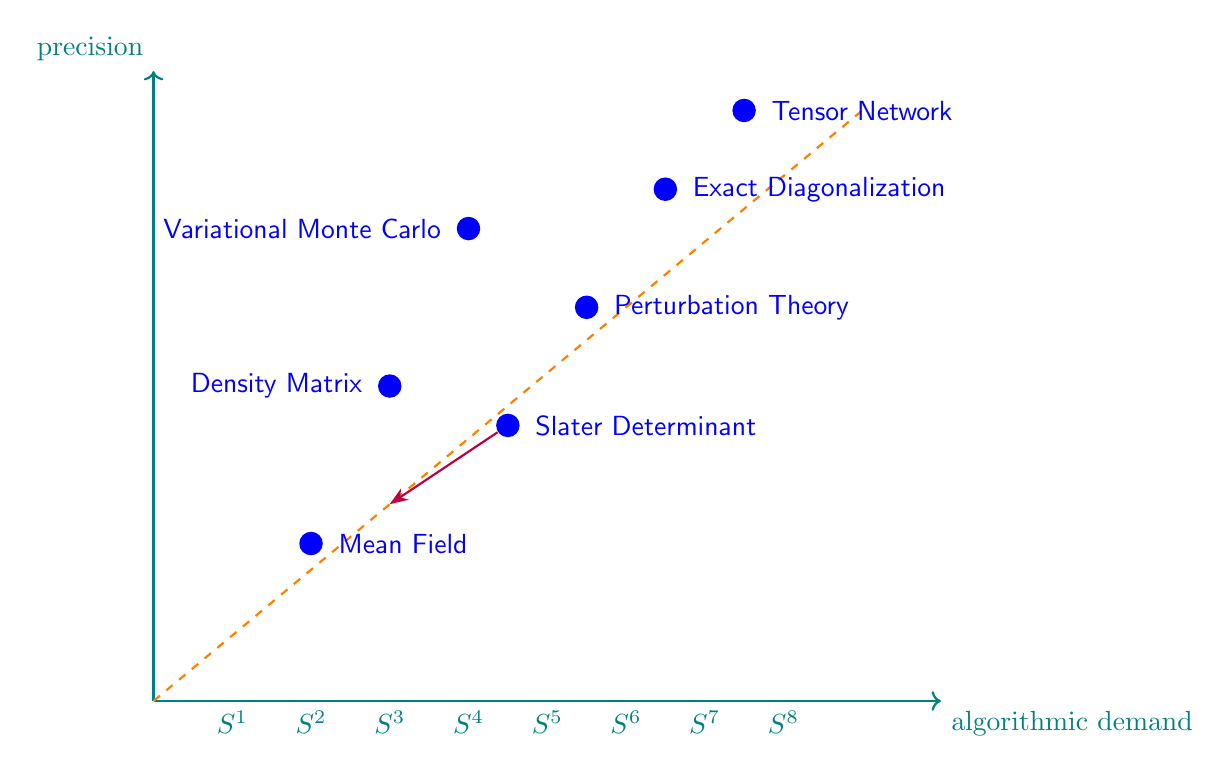
\begin{tikzpicture}[
    axis/.style={teal, thick, ->},
    label/.style={blue, font=\sffamily},
    point/.style={blue, circle, fill, inner sep=3pt},
    dashedline/.style={orange, dashed, thick},
    arrow/.style={purple, -{Stealth}, thick}
]

% Axes
\draw[axis] (0,0) -- (10,0) node[below right, teal] {algorithmic demand};
\draw[axis] (0,0) -- (0,8) node[above left, teal] {precision};

% X-axis labels
\foreach \i/\label in {1/S^1, 2/S^2, 3/S^3, 4/S^4, 5/S^5, 6/S^6, 7/S^7, 8/S^8} {
    \draw (\i,0) node[below, teal] {$\label$};
}

% Diagonal dashed line
\draw[dashedline] (0,0) -- (9,7.5);

% Data points and labels
\node[point] (mf) at (2,2) {};
\node[label, right=2pt of mf] {Mean Field};

\node[point] (dm) at (3,4) {};
\node[label, left=2pt of dm] {Density Matrix};

\node[point] (vmc) at (4,6) {};
\node[label, left=2pt of vmc] {Variational Monte Carlo};

\node[point] (sd) at (4.5,3.5) {};
\node[label, right=2pt of sd] {Slater Determinant};

\node[point] (pt) at (5.5,5) {};
\node[label, right=2pt of pt] {Perturbation Theory};

\node[point] (ed) at (6.5,6.5) {};
\node[label, right=2pt of ed] {Exact Diagonalization};

\node[point] (tn) at (7.5,7.5) {};
\node[label, right=2pt of tn] {Tensor Network};

% Purple arrow from Slater Determinant to Mean Field
\draw[arrow] (sd) -- ++(-1.5,-1) node[midway, above, purple] {};

\end{tikzpicture}
\end{document}